
\section{De Haas-va Alphen oscillation}

In this section the phenomenon of \ac{dHvA} oscillations is described. It is not immediately apparent how a ramping magnetic field could cause oscillations in such a wide range of parameters but Lifshitz and Kosevich provided an explanation through their eponymous equation based on a theoretical basis set out by Landau. This was then used to characterise the Fermi surface of many metals and establish the field of `Fermiology'. Strictly, only the oscillations in magnetisation are \ac{dHvA} oscillations and those in resistance are called Shubnikov-de Haas oscillations. Nonetheless they both originate from the same underlying phenomena of oscillations in the free energy of the system.

\subsection{Overview}

For metals, the majority of the interesting physics occurs at the Fermi level and, provided Fermi liquid theory holds true, the electrons at the Fermi level can be modelled to a high degree of accuracy with the Sommerfeld model --- that is a Fermi gas of non-interacting electrons in an infinite box. When a magnetic field is applied, the electrons have their usual grid pattern distribution of plane wave k-vectors rearranged such that the electrons move around orbital and helical paths. These rearranged k-vectors form a set of concentric tubes, known as Landau tubes, whose cross-sectional area, $a$, perpendicular to the field is given by the Onsager relation:\footnote{Derivations of the Onsager relation are given in several textbooks including pg. 32 of Schoenberg~\cite{Schoenberg1984} and pg. 272 of Ashcroft \& Mermin~\cite{Ashcroft1976}.} 
%%
\begin{equation}
\label{Eqn:Theo:Onsager}
\textit{a}_{k_{\perp}} = (r + 1/2)\frac{2\pi e B}{\hbar}
\end{equation}
%%
where $r$ is a quantisation number that sets apart each tube. We can see from the relation that as $\vect{B}$ increases, so does the cross-sectional area of the tubes. As the magnetic field is ramped, successive tubes periodically pass the Fermi surface causing a spike in the \ac{DOS} at the Fermi level and also oscillations in the energy of the system, $E$, which, for geometric reasons explained in the next section, are far stronger at the maximal and minimal (extremal) areas of Fermi surface. Thermodynamic quantities such as magnetic susceptibility ($\chi = \partial E/\partial B$) and heat capacity ($C_{V} = \partial^2E/\partial T^2|_{V}$) or quantities that depend on the \ac{DOS} at the Fermi level such as electrical resistance all oscillate as the field is ramped. Oscillations in the susceptibility are known as \ac{dHvA} oscillations, oscillations in the resistivity are known as Shubnikov-de Haas oscillations.

 We can relate the `frequency' $F$ (measured in $tesla$\footnote{n.b. that it is \emph{tesla} and not \emph{tesla$^{-1}$} because, as we shall see later, the oscillations are actually periodic in $1/B$ and \emph{not} $B$ so their frequency counterpart is measured in \emph{tesla}.}) that the tubes pass the Fermi surface to the extremal Fermi surface area using the following application of the Onsager relation,
%%
\begin{equation}
\textit{a}_{k_{\perp}} = \frac{2\pi e }{\hbar}F
\end{equation}
%%
By varying the direction of the field we can obtain a series of maximal and minimal Fermi surface areas in a variety of orientations in order to build a profile of the Fermi surface topology and size. In practice, there are many possible variations that might fit the model based on areas of cross-sectional slices alone and so typically ab-initio \ac{DFT} calculations --- described in sections~\ref{Sec:Theo:Dft} and~\ref{Sec:Exp:Dft} --- are employed to provide a basis which can be tweaked based on the constraints from the measurements. 

A more detailed analysis of this process follows, beginning with an illustrative mathematical treatment for oscillations in the magnetisation.

\subsection{Exploring the origin of the oscillations}

We begin by calculating the degeneracy of the Landau tubes i.e. the number of electron states per tube. Because the states under a magnetic field are a one-to-one rearrangement of the states with no field, we can use the Sommerfeld number of states per unit k-space ($V/4\pi^3$) to determine the degeneracy. From the Onsager relation (eqn.~\ref{Eqn:Theo:Onsager}) we see that the additional area for successive tubes is $\Delta a_{k_{\perp}}  = 2\pi e B/\hbar$ which we can convert to a volume by integrating over $k_{\perp}$. This gives a degeneracy per tube therefore of,

\begin{equation}
D_{\textrm{tube}} = d k_{\perp}\left(\frac{2\pi e B}{\hbar}\right)\left(\frac{V}{4 \pi^3}\right) = \frac{eBVdk_{\perp}}{\hbar 2\pi^2}
\end{equation}

We continue by writing an expression for the energy of the system, $E$ by summing the energies of the states that lie beneath the cross-sectional area defined by the Fermi surface ($a_{k_\perp F}$) for a given $k_\perp$. To do this, we use the Onsager equation to determine $R_\perp$ --- the number of Landau tubes below the Fermi surface at this cross-sectional slice. We then multiply this by the degeneracy of the tubes, $D$ and the energy for states on that particular Landau tube, $\epsilon_r$,
%%
\begin{equation}
\label{Eqn:Theo:OscillateE}
E = D\sum_{r}^{R_\perp}\epsilon_r = \frac{eBVdk_\perp}{\hbar 2 \pi^2}\sum_{r}^{R_\perp}\epsilon_r
\end{equation}
 where,
\begin{equation}
R_\perp = \textrm{floor}\left[\frac{a_{k_\perp F}\hbar}{2\pi e B} - \frac{1}{2}\right]
\end{equation}
%%
To complete the above equation, we need an expression for the energies of each of the Landau tubes. The procedure for the free electron case is to insert the canonical momentum (i.e momentum of a free electron in a magnetic field) into the non-interacting Schr\"odinger equation and solve to obtain the following eigenvalues for the energies on the Landau tubes. Full derivations can be found in several textbooks\footnote{See for examples pg. 32ff. in Schoenberg~\cite{Schoenberg1984} or pg. 148ff. in Blundell~\cite{Blundell2001}.} and so will  not be repeated here. Below is the expression for the energy eigenvalues,
%%
\begin{equation}
\epsilon_r=(r+1/2) \hbar \omega_c + \frac{\hbar^2 k^2}{2m_0} \textrm{\hspace{0.2cm}where,\hspace{0.2cm}} \omega_c = \frac{eB}{m_0}
\end{equation}
%%
and is known as the \emph{cyclotron frequency}. The summation term in equation~\ref{Eqn:Theo:OscillateE} can now be written,
%%
\begin{align*}
\sum_r^{R_\perp}\epsilon_r &= \sum_r^{R_\perp}\left( (r+1/2) \hbar \omega_c + \frac{\hbar^2 k^2}{2m_0} \right) \\
    &= \frac{\hbar eB}{m_0}\sum_r^{R_\perp}r + \frac{\hbar eB}{2m_0}\sum_r^{R_\perp}1 + \frac{\hbar^2 k^2}{2m_0}\sum_r^{R_\perp}1 \\
    &= \frac{\hbar eB}{2 m_0} R_\perp(R_\perp + 1) + \frac{\hbar eB}{2m_0}R_\perp + \frac{\hbar^2 k^2}{2m_0}R_\perp \\
    &= \frac{\hbar eB}{2m_0}R_\perp^2 + \left(\frac{\hbar eB}{m_0} + \frac{\hbar^2 k^2}{2m_0}\right)R_\perp
\end{align*}
%%
which can be expanded out and finally substituted back into equation~\ref{Eqn:Theo:OscillateE} to finally obtain,
%%
\begin{equation}
\label{Eqn:Theo:OscIllustration}
E = \frac{e^2Vdk_\perp}{4\pi^2m_0}B^2\left[R_\perp^2 + 2R_\perp + \frac{\hbar k^2}{e}\frac{1}{B}R_\perp\right]
\end{equation}
%%
Key to the above relation is that, although $R_\perp$ is inversely proportional to $B$, it remains discrete. This gives rise to the saw-tooth like function shown in figure~\ref{Fig:Theo:EnergyOscillations} for some typical experimental parameters. Also plotted is the function against $1/B$ where we can clearly see that the oscillations are periodic in inverse field hence the frequency being measured in tesla$^{-1}$.
%%
\begin{figure}[htbp]
    \begin{center}
        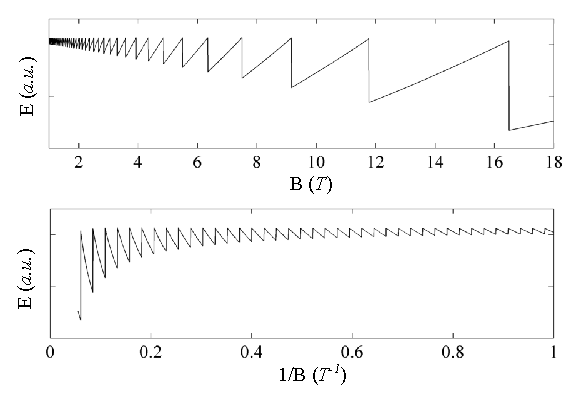
\includegraphics[scale=0.9]{Chapter-Theory/Figures/TheoreticalOscillations/TheoreticalOscillations}
        \caption{Theoretical energy oscillations for a Fermi surface orbit which is 5\% of a \unit{5}{\angstrom} cubic \ac{BZ} between \unit{1-18}{\tesla}. Kinetic energy term is taken to be for an electron at a level half the size of the Fermi surface.}
        \label{Fig:Theo:EnergyOscillations}
    \end{center}
\end{figure}

The above is not a rigorous derivation but is nonetheless illustrative of the origin of the oscillation in the system energy and how any thermodynamic value which depends on the energy of the system oscillates as a function of field. To continue we need to include correction factors to the oscillation amplitude due to finite electron scattering rates ($A_D$), temperature ($A_T$), Zeeman splitting of spins ($A_s$), doping ($A_{\textrm{dop}}$), mosaicity ($A_{\textrm{mos}}$), warping of the Fermi surface ($A_{\textrm{warp}}$) as well as adjustments due to the fact that the parameter measured was torque of the sample in a field and not the energy or magnetisation directly ($A_{\Gamma}$). For this, we turn to a more solid foundation that was put forward by Lifschitz and Kosevitch and presented by Schoenberg.

\subsection{\acl{LK} equation}

The derivation for the full expression for the Landau thermodynamic potential, $\Omega$\footnote{Formally defined as the energy in a open system that is in thermal contact with its surroundings}, begins in a similar way to the previous illustrative example but frames the sawtooth-like function above as a more mathematically manageable Fourier decomposition which also conveniently makes the technique highly amenable to Fourier analysis. For this reason the equation below features higher harmonics which are denoted with the identifier $p$.
%%
\begin{equation}
\Omega = \left(\frac{e}{2\pi\hbar}\right)^{\frac{3}{2}}\frac{e\hbar B^{\frac{5}{2}}}{m_0 \pi^2}\left| \frac{\partial^2 a_{\textrm{ext}}}{\partial k^2_\perp}\right|^{-\frac{1}{2}}\sum_{p=1}^{\infty}p^{-\frac{5}{2}}A_{\textrm{tot}}\cos\left[2\pi p\left(\frac{F}{B} - \gamma\right)\pm\frac{\pi}{4}\right]
\end{equation}
where,
\begin{equation}
A_{\textrm{tot}} = A_T A_D A_s A_{\Gamma} A_{\textrm{mos}} A_{\textrm{dop}} A_{\Delta B}
\end{equation}
%%
The above equation and derivatives of it are known as the \ac{LK} equation. To obatin the magnetisation the differential with respect to $b$ is taken to get,
%%
\begin{equation}
M = \left(\frac{e}{\hbar}\right)^{\frac{3}{2}}\frac{e\hbar F V B^{\frac{1}{2}}}{m_0 \pi^\frac{5}{2}\sqrt{2}}\left| \frac{\partial^2 a_{\textrm{ext}}}{\partial k^2_\perp}\right|^{-\frac{1}{2}}\sum_{p=1}^{\infty}p^{-\frac{3}{2}}A_{\textrm{tot}}\sin\left[2\pi p\left(\frac{F}{B} - \gamma\right)\pm\frac{\pi}{4}\right]
\end{equation}
%%
To attain the above equations, it was necessary to perform an integral over $k_\perp$\footnote{Similar to the integral in the toy equation from the previous section} which results in a parameter for an extremal Fermi surface orbit area perpendicular to the field given by $a_{\textrm{ext}}$. 

\subsubsection{Attenuation for non-extremal orbits}

Only the extremal (i.e. the largest and smallest) magnetically induced orbits contribute significantly to oscillations in the system energy. This is because $F$ represents a phase factor in the \ac{LK} equation and at the extremal points $dF/dk_\perp=0$ meaning more orbits near extrema are in phase. However it is not immediately clear how much stronger the oscillations from the extremal orbits will be in comparison to other orbits. Figure~\ref{Fig:Theo:ExtremalPhases} shows examples of the strengths of the oscillations after integrating over a distribution of phases shown in the insets.
%%
\begin{figure}[htbp]
    \begin{center}
        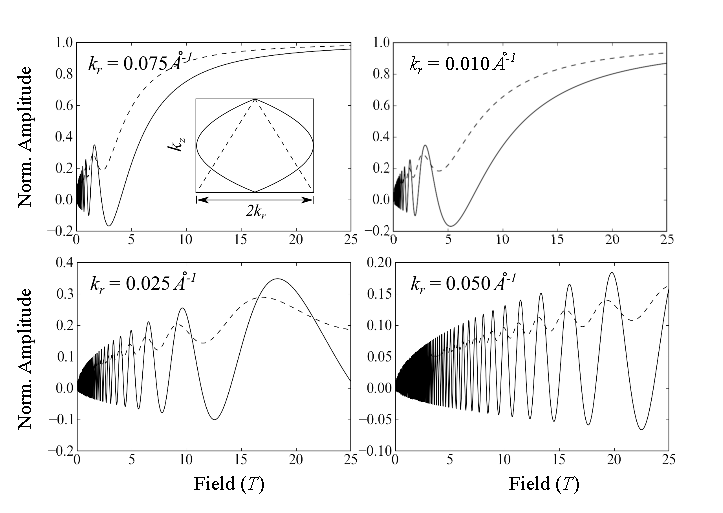
\includegraphics[scale=0.8]{Chapter-Theory/Figures/ExtremalPhases/ExtremalPhases}
        \caption{The sum of 1000 cosines with phase dispersions shown in the insets. Dashed line represents an extremal dispersion, solid lines a spread of linear dispersions and dotted line represent a non-extremal inflection point. Top left, top right and bottom left panels have phase distributions that are scaled from $0$ to $\sim1$, $\approx10$ and $\approx100$ Landau tube `wavelengths' respectively.}
        \label{Fig:Theo:ExtremalPhases}
    \end{center}
\end{figure}
%%
The panels each show the phases from the distributions taken over a range of scales, and it is clear that the phase cancellation is more acute for longer scales. This makes sense if we consider that the Landau tubes passing the Fermi surface are a oscillatory measurement probe like any other and so will be wavelength limited. That is, if the difference between the outermost and innermost orbits are of the order of the Landau tube spacing as is passes the Fermi surface, then the oscillations will be difficult to pick out. Interestingly this also places a limit on the maximum field that can be used to probe a Fermi surface since, according to the Onsager relation, the larger the field the larger the spacing between tubes. In practice this is simply $\Delta a_{k_\perp}$ which means that in terms of $F$, the resolutions is simply the field (i.e. $\sigma_F \sim \unit{18}{\tesla}$ for the Yellow magnet at Bristol). 

A final point is that it is not strictly extremal points that contribute significantly to the oscillations, but also inflected stationary points as shown in the last panel of figure~\ref{Fig:Theo:ExtremalPhases} so on could imagine a pathological stepped Fermi surface that would feature several strong orbital oscillations which would not be at turning points.

Variations in the phases can also be put into practice to model the various effects on the \ac{LK} equation listed towards the end of the previous section. These can be manifest by convolving an appropriate phase distribution function with the cosine oscillatory term. It can be shown\footnote{See for example, Schoenberg pg 57--59.~\cite{Schoenberg1984}} that this convolution results in a relatively simple multiplication factor --- hence the various $A$ factors listed in the \ac{LK} equation which we expand upon below.

\subsubsection{Attenuation due to temperature}

To find the appropriate phase distribution function for the temperature dependence we start with the Fermi distribution,
\begin{equation}
\label{Eqn:Theo:FermiFunction}
f(\epsilon) = \frac{1}{\exp\left((\epsilon-\mu)/kT\right) + 1}
\end{equation} 
The differential of this distribution results in the broadening function (which is proportional to the probability that the Fermi energy $\mu$ is between $\epsilon$ and $\epsilon + d\epsilon$),
\begin{equation}
  P(\epsilon < \mu < \epsilon + d\epsilon) \propto \frac{d\epsilon}{2kT(1 + \cosh[(\epsilon - \mu)/kT])}
\end{equation}
This is convolved across the Fermi energy to smear it and also the phase through the parameter $F$. The details of how this is done is given in Schoenberg pg. 59ff~\cite{Schoenberg1984} with the end result is given by,
\begin{equation}
\label{Eqn:Theo:TemperatureTerm}
  A_T = \frac{X}{\sinh(X)} \textrm{\hspace{0.3cm} where,\hspace{0.3cm}} X = \frac{2\pi^2pkT m^*_T}{e\hbar B}
\end{equation}

The above factor includes $m^*_T$, the \emph{thermal effective mass} as a term in a function of $T$. As a consequence, by studying the temperature dependence of the amplitude it is possible to get a measure of $m^*_T$ of the electrons at the extremal orbit. Techniques for doing this are discussed in section~\ref{Sec:Exp:ExtractingEffMassTemperatureDependence}.

The effective mass determined in this way is enhanced subject to the same interactions as in heat capacity experiments --- i.e. electron-phonon interactions and spin symmetric correlations --- but are probed for a particular Fermi surface orbit, whereas heat capacity is bulk averaged. As we will see later the mass enhancement is is different to that from spin measurements. For more one this see Rourke \etal~\cite{Rourke2010b} and references therein.

\subsubsection{Attenuation due to finite quasiparticle lifetime}

The \emph{Dingle factor}, $A_D$, is due to the finite lifetime, $\tau$, of the electron quasiparticles due to scattering. Because of this time scale, there is a smearing of the electron energy through the uncertainty principle with a broadening which is approximately Lorentzian in shape. If we assume $\tau$ does not change with energy\footnote{This is not the case, but at most only a few Landau levels contribute to a particular oscillation and if we assume that the energy does not vary too much between subsequent levels then the assumption is a good one}, then this can be modelled as a smearing of the Fermi level such that the broadening function is,
\begin{equation}
  P(\epsilon < \mu < \epsilon + d\epsilon) \propto \frac{d\epsilon}{(\epsilon - \mu)^2 + (\hbar/2\tau)^2}
\end{equation}
and such that after the routine Fourier transform, the end relation is given by,
\begin{equation}
  A_D = e^{-\pi p m_b/e B\tau} = e^{-\pi p/\omega_c\tau} 
\label{Eqn:Theo:DingleTerm}
\end{equation}
The exponent in the above can be thought of as the number of orbits the electron has completed (i.e. each harmonic $p$ is another successive orbit) divided by the expected number of orbits it will complete, so evidently we expect to see the higher harmonics having an exponentially lower amplitude. The term $m_b$ refers to the \emph{band mass} which will be discussed in detail later on. 
%The mass term here is \TODO{How is it coupled as Tony described?}

\subsubsection{Attenuation due to spin splitting}

Applying a magnetic field causes a Zeeman splitting of energy levels of magnitude,
\begin{equation}
  \Delta\epsilon = \frac{g e \hbar B}{2 m_e}
\end{equation}
where $m_e$ is the free electron mass and $g$ is a factor that is $\approx2$ for free electrons. Rather than smearing, this can be thought of as two separate Fermi surfaces with separate Fermi energies. The attenuation is given then as,
\begin{equation}
  A_s = \cos\left(\frac{\pi p g m^*_s}{2m_e}\right)
\end{equation}
where $m^*_s$ is the \emph{spin effective mass}. This is subject to a different set of interaction in comparison to the thermal effective mass -- notably both spin symmetric and antisymmetric correlations but not the electron-phonon interactions. As such, in materials with strong phonon interactions we may see a strong difference in $m^*_s$ and $m^*_T$.

\subsubsection{Other attenuating factors}

Another attenuating factor due to slight misalignments in the crystal structure, ($A_{mos}$), causing a mosaic polycrystalline structure could be modelled with an appropriate broadening function. Schoenberg suggests a Lorentzian similar to the Dingle factor --- there is no solid mathematical basis for this but no other function shape has been observed in experiment. The final form would then look like the following,
\begin{equation}
  A_{\textrm{mos}} = e^{2\pi p \Delta F_{\textrm{mos}}/B}
\end{equation}
where $\Delta F_{mos}$ is a parameter that determines the degree of overall misalignment.

The final attenuating factors mentioned here are $A_{\Delta B}$, the damping due to field inhomogeneity which has an effect depending on the shape of the field and $A_{\textrm{dop}}$, which is another Lorentzian-like broadening factor due to the doping inhomogeneity in the sample. Neither of which will be considered in the thesis --- the material studied is undoped, and the magnet is suitably large as to have an essentially linear field profile ---doping and so will not be explored further\footnote{If you do want to consider these factors, ref~\cite{Rourke2010b} has a passage on doping homogeneity and pg. 64 of Schoenberg discusses field inhomogeneity~\ref{Schoenberg1984}.}

\subsection{Zeeman-Doppler shifting of oscillations}

One ramification of the spin splitting is that as the field ramps there is a gradual increase and/or decrease in the size of the split Landau levels commensurate with field with $\Delta a \propto B$. In a paramagnetic material we expect there to be a majority of spins aligned with the field meaning the Fermi surface will mostly shrink as the field ramps in one direction and expand as it ramps in the opposite direction. This leads to an apparent extra shift in the frequency which is proportional to $B$ which is of order of the field strength.


\subsection{Band mass}

So far, three different electron masses have been defined, the thermal effective mass, the spin effective mass and the free electron mass. To tie these together a fourth mass is introduced, the \emph{band mass}. This is another effective mass resulting from the electrons being subject to the bandstructure potential as defined by \ac{DFT} calculations and is given by,
\begin{equation}
  m^*_b = \hbar^2 \left(\frac{d^2\epsilon}{dk^2}\right)^{-1} = \frac{\hbar^2}{2\pi}\frac{\partial a_{k_\perp}}{\partial \epsilon}
\end{equation}
Mass enhancement comes from any kind of interactions the electron has with its environment --- i.e. external fields, other electrons and nuclei --- resulting in the free electron mass $m_e$ becoming enhanced (renormalised). The bands mass can be determined from \ac{DFT} and the resulting enhancement is purely from the interaction of the electron with the calculated lattice potential. However \ac{DFT} calculations typically do not model correlation effects well or dynamic interactions at all. We know that both the thermal effective mass and the spin effective mass incorporate the band mass enhancements plus a unique set of interactions specified previously. Figure~\ref{Fig:Theo:EffectiveMassInheritance} lays out how the effective masses build on each other by incorporating more interactions.
\begin{figure}[htbp]
    \begin{center}
        \includegraphics[scale=0.9]{Chapter-Theory/Figures/EffectiveMassInheritance/EffectiveMassInheritance}
        \caption{A diagram showing how the successive electron masses build on the previous interactions. Additional interaction effects are listed in italics.}
        \label{Fig:Theo:EffectiveMassInheritance}
    \end{center}
\end{figure}
because of this particular hierarchy, it is sometimes possible to compare effective masses to get a sense of scale of the interactions.

\subsubsection{A 2D Approximation}

Although none of the attenuating factors above have an explicit angle dependence, they do vary as a function of angle through the band mass. A common approximation to simulate the dependency in layered systems is to assume the Fermi surface is two dimensional in shape and therefore cylindrical. The cross section of a cylinder is given by,
\begin{equation}
    a = \frac{a_0}{\cos \theta},
\end{equation}
where $\theta$ is the angle from the cylinder axis. Increasing the Fermi energy by $\Delta \epsilon$ will cause the cross section at zero angle to change by amount $\Delta a_0$, then the band mass is given by,
\begin{equation}
    m^*_b = \frac{\hbar^2}{2\pi}\frac{\partial a_{k_\perp}}{\partial \epsilon} = \frac{\hbar^2}{2\pi}\frac{\partial}{\partial \epsilon}\left(\frac{a_0 + \Delta a_0 }{\cos\theta} - \frac{a_0 }{\cos\theta}\right) = \frac{\hbar^2}{2\pi}\frac{\partial a_0}{\partial \epsilon}\frac{1}{\cos \theta},
\end{equation}
therefore
\begin{equation}
    m^*_b = \frac{m^*_{b0} }{\cos{\theta}}
\end{equation}
This means that under this approximation, any factor that includes the band mass, explicitly or implicitly\footnote{Meaning $m^*_T$ and $m^*_S$ which are both enhancements of the band mass} can be resolved using the zero angle band mass with an angle dependence of $1/\cos{\theta}$.

\subsection{Final theoretical observations}

Originally \ac{dHvA} measurements were used to measure the Fermi surfaces of elemental metals and so the initial assumption of a free-electron gas is justified based on the fact that elemental metals have a Fermi surface and are considered materials that adhere to Fermi liquid theory. The fact that oscillations have been observed in cuprates and pnictides which have demonstrated non-Fermi liquid behaviour is therefore remarkable and moreover implies the presence of a Fermi surface, at least in the presence of a strong magnetic field.

